% HG-DAgger / Online-RL system architecture -- FFW SG2 + A2 leader
% Compile: pdflatex, xelatex or tectonic. No exotic packages.
%
% LAYOUT NOTE (2026-08-30 rewrite)
% The previous version put the runtime control path and the recording/conversion
% path on one a3 canvas. That forced every cross-container edge through the same
% narrow corridor and several labels landed on node text: T15/T1 crossing on the
% left, T14 over the broadcaster, "policy input drops it" struck through by an
% edge, T10 over the browser caption, the cyclo container label colliding.
%
% This version separates the two concerns:
%   page 1  RUNTIME  -- who commands the arms, and how control is handed over
%   page 2  DATA     -- what is recorded and what survives conversion
%   page 3+ LEGEND   -- every topic and service, type and semantics
%
% Nodes sit on an ABSOLUTE grid (x=1cm, y=1cm) rather than relative
% "below=of" chains, so one node can be nudged without cascading through
% everything downstream. Cross-container edges leave from a named anchor and
% turn in open space rather than over a node.
\documentclass{article}
\usepackage[a3paper,landscape,margin=1.2cm]{geometry}
\usepackage{tikz}
\usepackage{graphicx}
\usepackage{longtable}
\usepackage{enumitem}
\usetikzlibrary{positioning,arrows.meta,fit,backgrounds,calc}
\usepackage{helvet}
\renewcommand{\familydefault}{\sfdefault}
\usepackage{xcolor}
\pagestyle{empty}
\setlength{\parindent}{0pt}

\definecolor{cAiWorker}{RGB}{225,240,255}
\definecolor{cCyclo}{RGB}{255,238,215}
\definecolor{cPolicy}{RGB}{232,225,255}
\definecolor{cUI}{RGB}{225,250,230}
\definecolor{cDisk}{RGB}{238,238,238}
\definecolor{cBad}{RGB}{255,226,226}
\definecolor{eHuman}{RGB}{178,58,58}
\definecolor{eAuto}{RGB}{38,108,188}
\definecolor{eData}{RGB}{95,95,95}

\tikzset{
  proc/.style   ={draw,rounded corners=2pt,align=center,font=\small,
                  minimum height=9mm,inner sep=3pt,fill=white},
  hw/.style     ={draw,dashed,rounded corners=2pt,align=center,font=\small,
                  minimum height=8mm,inner sep=3pt,fill=white},
  disk/.style   ={draw,align=center,font=\small,fill=cDisk,inner sep=3pt},
  bad/.style    ={draw,align=center,font=\small,fill=cBad,inner sep=3pt,thick},
  container/.style={draw,rounded corners=4pt,inner sep=5mm,line width=0.4pt},
  ed/.style     ={-{Stealth[length=2mm]},draw=eData,line width=0.5pt},
  human/.style  ={-{Stealth[length=2mm]},draw=eHuman,line width=1.1pt},
  auto/.style   ={-{Stealth[length=2mm]},draw=eAuto,line width=1.1pt},
  lbl/.style    ={font=\scriptsize,fill=white,inner sep=1pt},
  note/.style   ={font=\scriptsize\itshape,align=left},
}

\begin{document}

% =====================================================================
% PAGE 1 -- RUNTIME
% =====================================================================
\begin{center}
{\LARGE\bfseries HG-DAgger / Online-RL --- Runtime Control Path}\\[1mm]
{\small FFW SG2 follower $\cdot$ A2 leader $\cdot$ GR00T-N1.7 policy}\\[1.5mm]
{\footnotesize\itshape
\textcolor{eHuman}{\rule{5mm}{1.2pt}}~human commands the arms \quad
\textcolor{eAuto}{\rule{5mm}{1.2pt}}~policy commands the arms \quad
\textcolor{eData}{\rule{5mm}{0.6pt}}~status / feedback / control plane.
\ Edge labels are IDs defined in the legend on p.3.}
\end{center}
\vspace{1mm}

% width capped at 0.86 so the SCALED HEIGHT still fits the a3 text block --
% \resizebox constrains one dimension only, and at full \textwidth this
% picture's height overflowed and the page came out blank.
\resizebox{0.86\textwidth}{!}{%
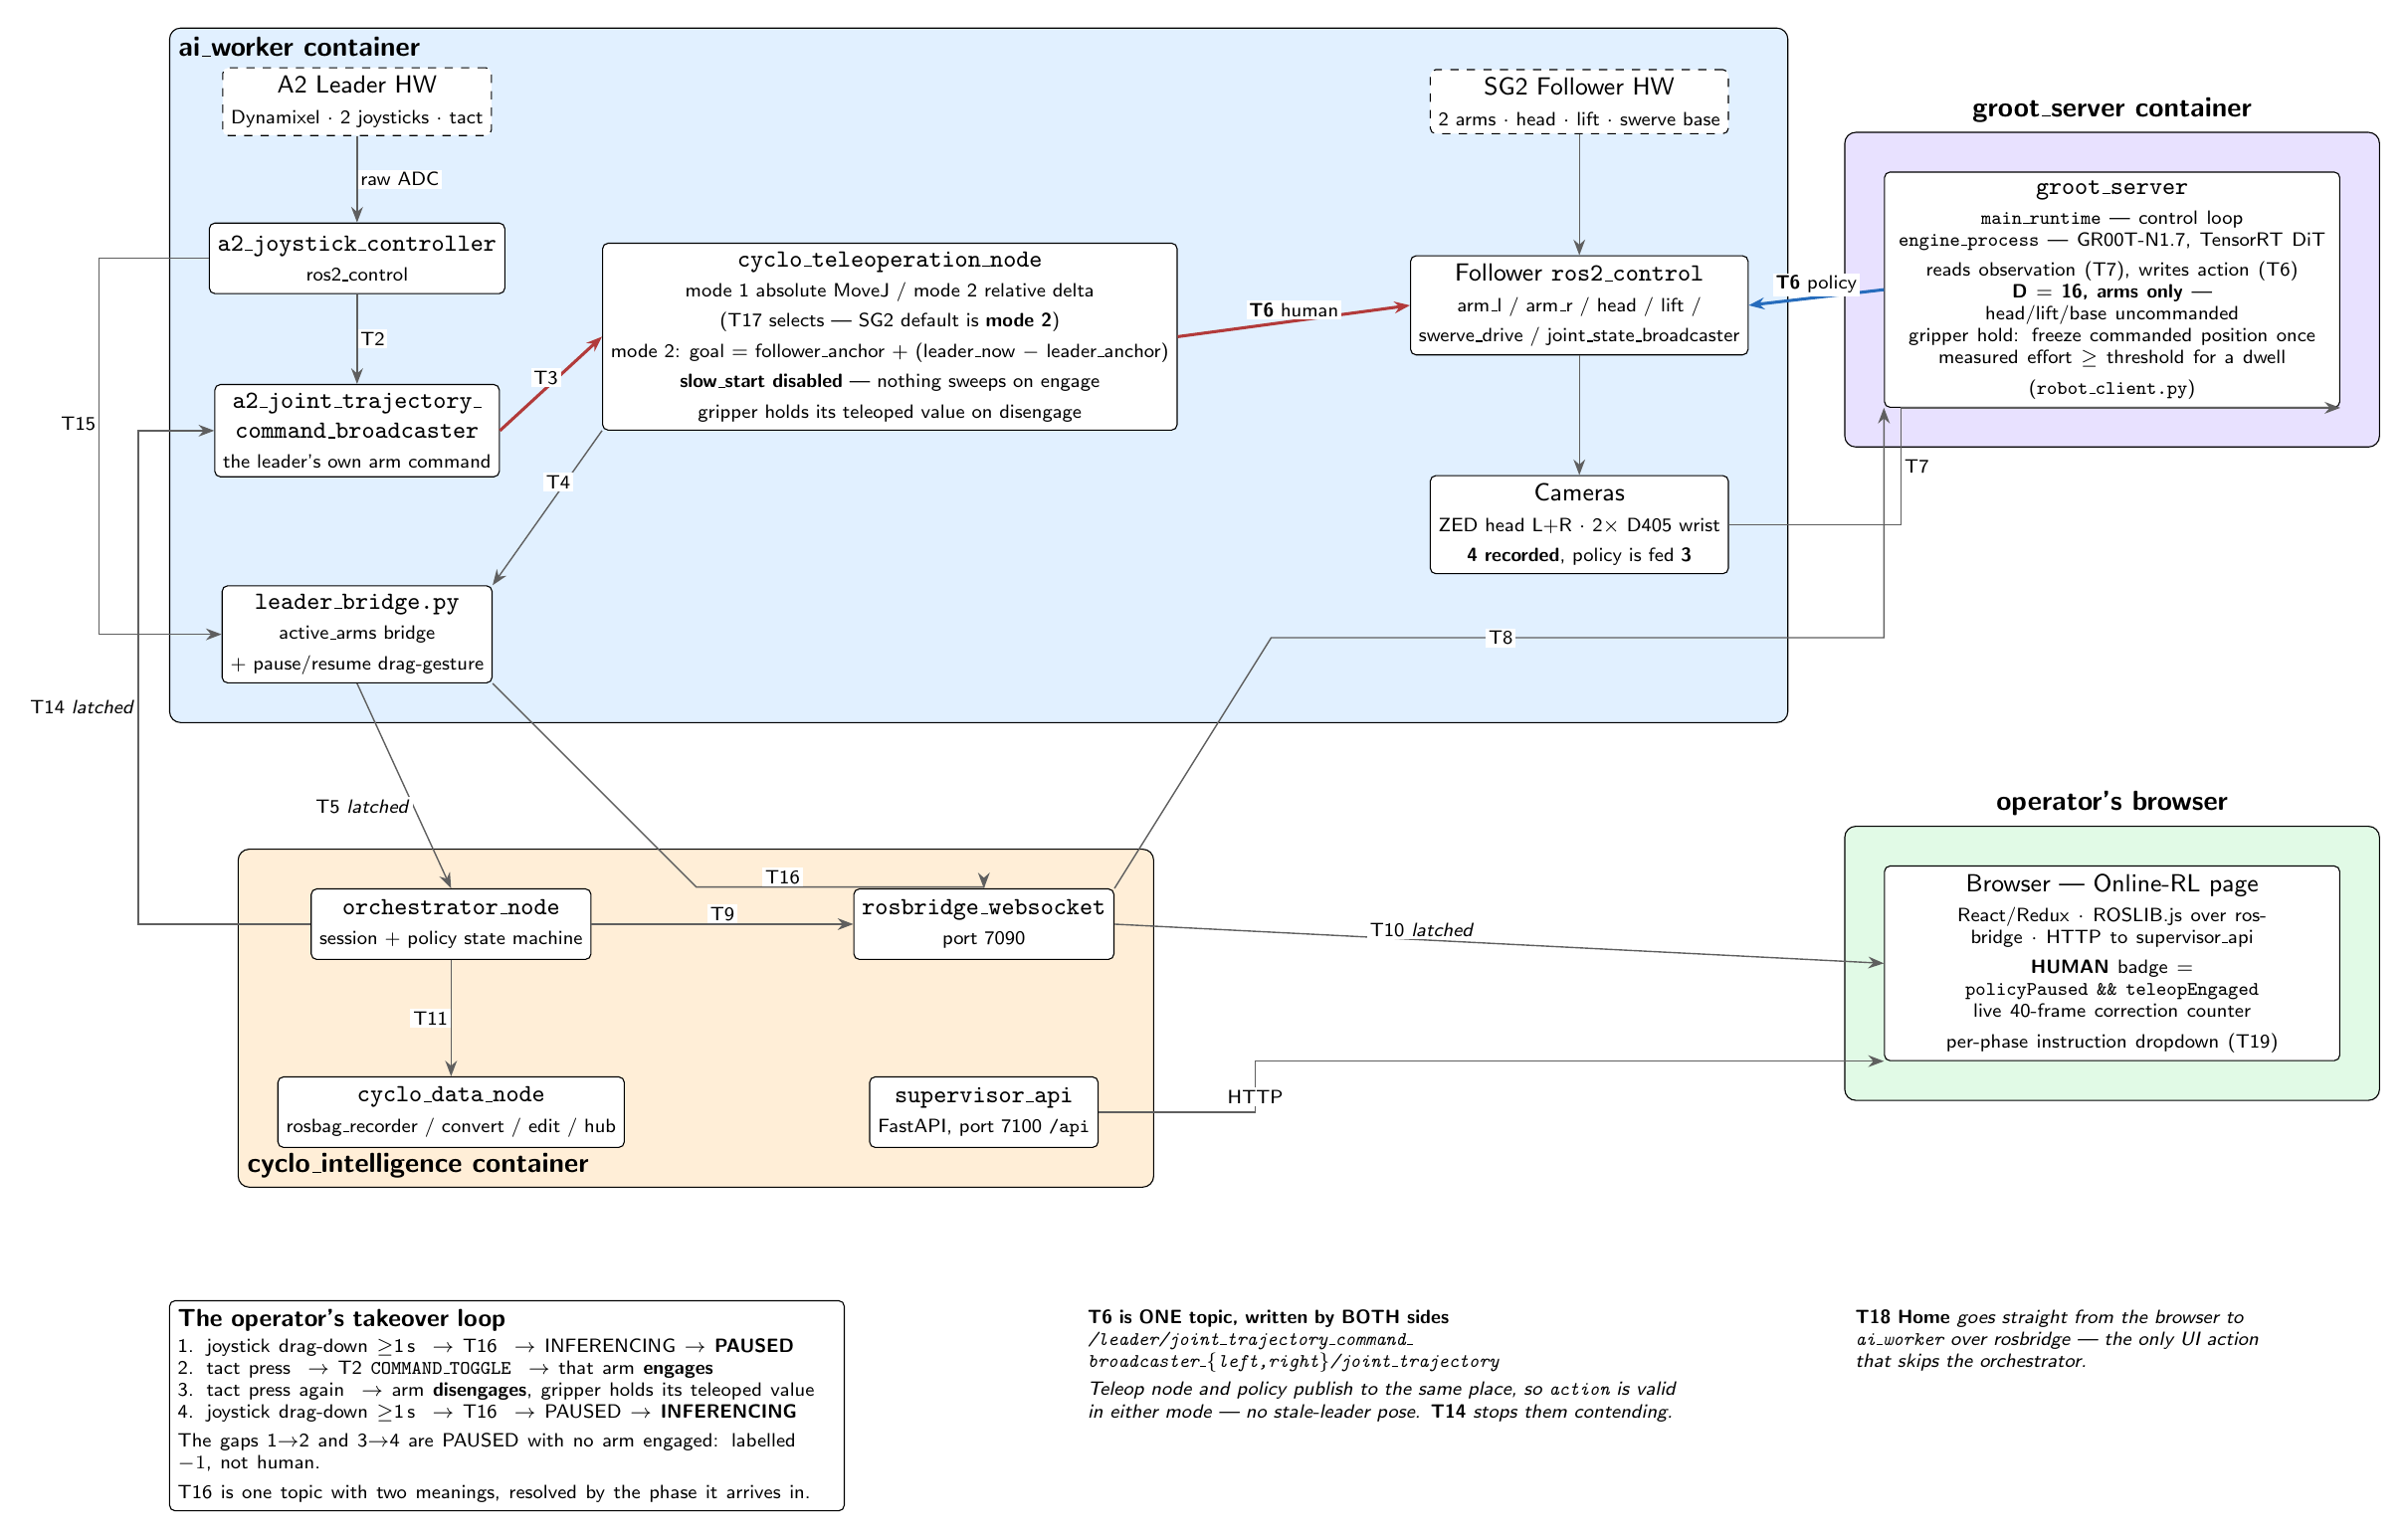
\begin{tikzpicture}[x=1cm,y=1cm]

% ---------- ai_worker: leader chain ----------
\node[hw]   (lhw)    at ( 2.6,14.4) {A2 Leader HW\\\scriptsize Dynamixel $\cdot$ 2 joysticks $\cdot$ tact};
\node[proc] (joy)    at ( 2.6,12.4) {\texttt{a2\_joystick\_controller}\\\scriptsize ros2\_control};
\node[proc] (bcast)  at ( 2.6,10.2) {\texttt{a2\_joint\_trajectory\_}\\\texttt{command\_broadcaster}\\\scriptsize the leader's own arm command};
\node[proc] (bridge) at ( 2.6, 7.6) {\texttt{leader\_bridge.py}\\\scriptsize active\_arms bridge\\\scriptsize + pause/resume drag-gesture};

% ---------- ai_worker: teleop + follower ----------
\node[proc] (teleop) at ( 9.4,11.4) {\texttt{cyclo\_teleoperation\_node}\\\scriptsize mode 1 absolute MoveJ / mode 2 relative delta\\\scriptsize (T17 selects --- SG2 default is \textbf{mode 2})\\\scriptsize mode 2: goal $=$ follower\_anchor $+$ (leader\_now $-$ leader\_anchor)\\\scriptsize \textbf{slow\_start disabled} --- nothing sweeps on engage\\\scriptsize gripper holds its teleoped value on disengage};
\node[hw]   (fhw)    at (18.2,14.4) {SG2 Follower HW\\\scriptsize 2 arms $\cdot$ head $\cdot$ lift $\cdot$ swerve base};
\node[proc] (fctrl)  at (18.2,11.8) {Follower \texttt{ros2\_control}\\\scriptsize arm\_l / arm\_r / head / lift /\\\scriptsize swerve\_drive / joint\_state\_broadcaster};
\node[proc] (cams)   at (18.2, 9.0) {Cameras\\\scriptsize ZED head L+R $\cdot$ 2$\times$ D405 wrist\\\scriptsize \textbf{4 recorded}, policy is fed \textbf{3}};

\begin{scope}[on background layer]
\node[container,fill=cAiWorker,
      fit=(lhw)(joy)(bcast)(bridge)(teleop)(fhw)(fctrl)(cams),
      label={[font=\bfseries,anchor=north west]north west:ai\_worker container}] (awbox) {};
\end{scope}

% ---------- groot_server ----------
\node[proc,text width=56mm] (policy) at (25.0,12.0)
  {\texttt{groot\_server}\\[1mm]
   \scriptsize\texttt{main\_runtime} --- control loop\\
   \scriptsize\texttt{engine\_process} --- GR00T-N1.7, TensorRT DiT\\[1mm]
   \scriptsize reads observation (T7), writes action (T6)\\
   \scriptsize \textbf{D $=$ 16, arms only} --- head/lift/base uncommanded\\
   \scriptsize gripper hold: freeze commanded position once\\
   \scriptsize measured effort $\geq$ threshold for a dwell\\
   \scriptsize (\texttt{robot\_client.py})};
\begin{scope}[on background layer]
\node[container,fill=cPolicy,fit=(policy),
      label={[font=\bfseries]north:groot\_server container}] (pbox) {};
\end{scope}

% ---------- cyclo_intelligence ----------
\node[proc] (orch)   at ( 3.8, 3.9) {\texttt{orchestrator\_node}\\\scriptsize session + policy state machine};
\node[proc] (rb)     at (10.6, 3.9) {\texttt{rosbridge\_websocket}\\\scriptsize port 7090};
\node[proc] (cdata)  at ( 3.8, 1.5) {\texttt{cyclo\_data\_node}\\\scriptsize rosbag\_recorder / convert / edit / hub};
\node[proc] (supapi) at (10.6, 1.5) {\texttt{supervisor\_api}\\\scriptsize FastAPI, port 7100 \texttt{/api}};
\begin{scope}[on background layer]
\node[container,fill=cCyclo,fit=(orch)(rb)(cdata)(supapi),
      label={[font=\bfseries,anchor=south west]south west:cyclo\_intelligence container}] (cbox) {};
\end{scope}

% ---------- browser ----------
\node[proc,text width=56mm] (ui) at (25.0,3.4)
  {Browser --- Online-RL page\\[1mm]
   \scriptsize React/Redux $\cdot$ ROSLIB.js over rosbridge $\cdot$ HTTP to supervisor\_api\\[1mm]
   \scriptsize \textbf{HUMAN} badge $=$ \texttt{policyPaused \&\& teleopEngaged}\\
   \scriptsize live 40-frame correction counter\\
   \scriptsize per-phase instruction dropdown (T19)};
\begin{scope}[on background layer]
\node[container,fill=cUI,fit=(ui),
      label={[font=\bfseries]north:operator's browser}] (uibox) {};
\end{scope}

% ---------- leader chain ----------
\draw[ed]    (lhw)   -- node[lbl,right]{raw ADC} (joy);
\draw[ed]    (joy)   -- node[lbl,right]{T2} (bcast);
\draw[human] (bcast.east) -- node[lbl,above,pos=0.45]{T3} (teleop.west);
\draw[ed]    (joy.west)   -- ++(-1.4,0) |- node[lbl,pos=0.22,left]{T15} (bridge.west);
\draw[ed]    (teleop.south west) -- node[lbl,above,pos=0.4]{T4} (bridge.north east);

% ---------- the shared action topic ----------
\draw[human] (teleop.east) -- node[lbl,above,pos=0.5]{\textbf{T6} human} (fctrl.west);
\draw[auto]  (policy.west) -- node[lbl,above,pos=0.5]{\textbf{T6} policy} (fctrl.east);

\node[note,text width=76mm,anchor=north west] at (11.8,-0.9)
 {\textbf{T6 is ONE topic, written by BOTH sides}\\
  \texttt{\scriptsize /leader/joint\_trajectory\_command\_}\\
  \texttt{\scriptsize broadcaster\_\{left,right\}/joint\_trajectory}\\[0.8mm]
  Teleop node and policy publish to the same place, so \texttt{action} is valid in either
  mode --- no stale-leader pose. \textbf{T14} stops them contending.};

% ---------- follower feedback ----------
\draw[ed] (fhw)   -- (fctrl);
\draw[ed] (fctrl) -- (cams);
\draw[ed] (cams.east) -- ++(2.2,0) |- node[lbl,pos=0.25,right]{T7} (policy.south east);

% ---------- control plane ----------
\draw[ed] (orch.west)   -- ++(-2.2,0) |- node[lbl,pos=0.22,left]{T14 \emph{latched}} (bcast.west);
\draw[ed] (bridge.south) -- node[lbl,left,pos=0.6]{T5 \emph{latched}} (orch.north);
\draw[ed] (bridge.south east) -- ++(2.6,-2.6) -| node[lbl,pos=0.15,above]{T16} (rb.north);
\draw[ed] (orch) -- node[lbl,above]{T9} (rb);
\draw[ed] (rb.east) -- node[lbl,above,pos=0.4]{T10 \emph{latched}} (ui.west);
\draw[ed] (orch.south) -- node[lbl,left]{T11} (cdata.north);
\draw[ed] (supapi.east) -- ++(2.0,0) |- node[lbl,pos=0.25,below]{HTTP} (ui.south west);
\draw[ed] (rb.north east) -- ++(2.0,3.2) -| node[lbl,pos=0.2,left]{T8} (policy.south west);

\node[note,text width=56mm,anchor=north west] at (21.6,-0.9)
 {\textbf{T18 Home} goes straight from the browser to \texttt{ai\_worker}
  over rosbridge --- the only UI action that skips the orchestrator.};

\node[proc,text width=84mm,align=left,anchor=north west] at (0.2,-0.9)
 {\textbf{The operator's takeover loop}\\[0.5mm]
  \scriptsize 1. joystick drag-down $\geq$1\,s \ $\to$ T16 \ $\to$ INFERENCING $\to$ \textbf{PAUSED}\\
  \scriptsize 2. tact press \ $\to$ T2 \texttt{COMMAND\_TOGGLE} \ $\to$ that arm \textbf{engages}\\
  \scriptsize 3. tact press again \ $\to$ arm \textbf{disengages}, gripper holds its teleoped value\\
  \scriptsize 4. joystick drag-down $\geq$1\,s \ $\to$ T16 \ $\to$ PAUSED $\to$ \textbf{INFERENCING}\\[0.8mm]
  \scriptsize The gaps 1$\to$2 and 3$\to$4 are PAUSED with no arm engaged: labelled $-1$, not human.\\
  \scriptsize T16 is one topic with two meanings, resolved by the phase it arrives in.};

\end{tikzpicture}}

\newpage

% =====================================================================
% PAGE 2 -- DATA
% =====================================================================
\begin{center}
{\LARGE\bfseries Recording and Conversion --- what survives to training}\\[1mm]
{\small Every recorded topic, and where the online-RL labels are lost}
\end{center}
\vspace{1mm}

\resizebox{\textwidth}{!}{%
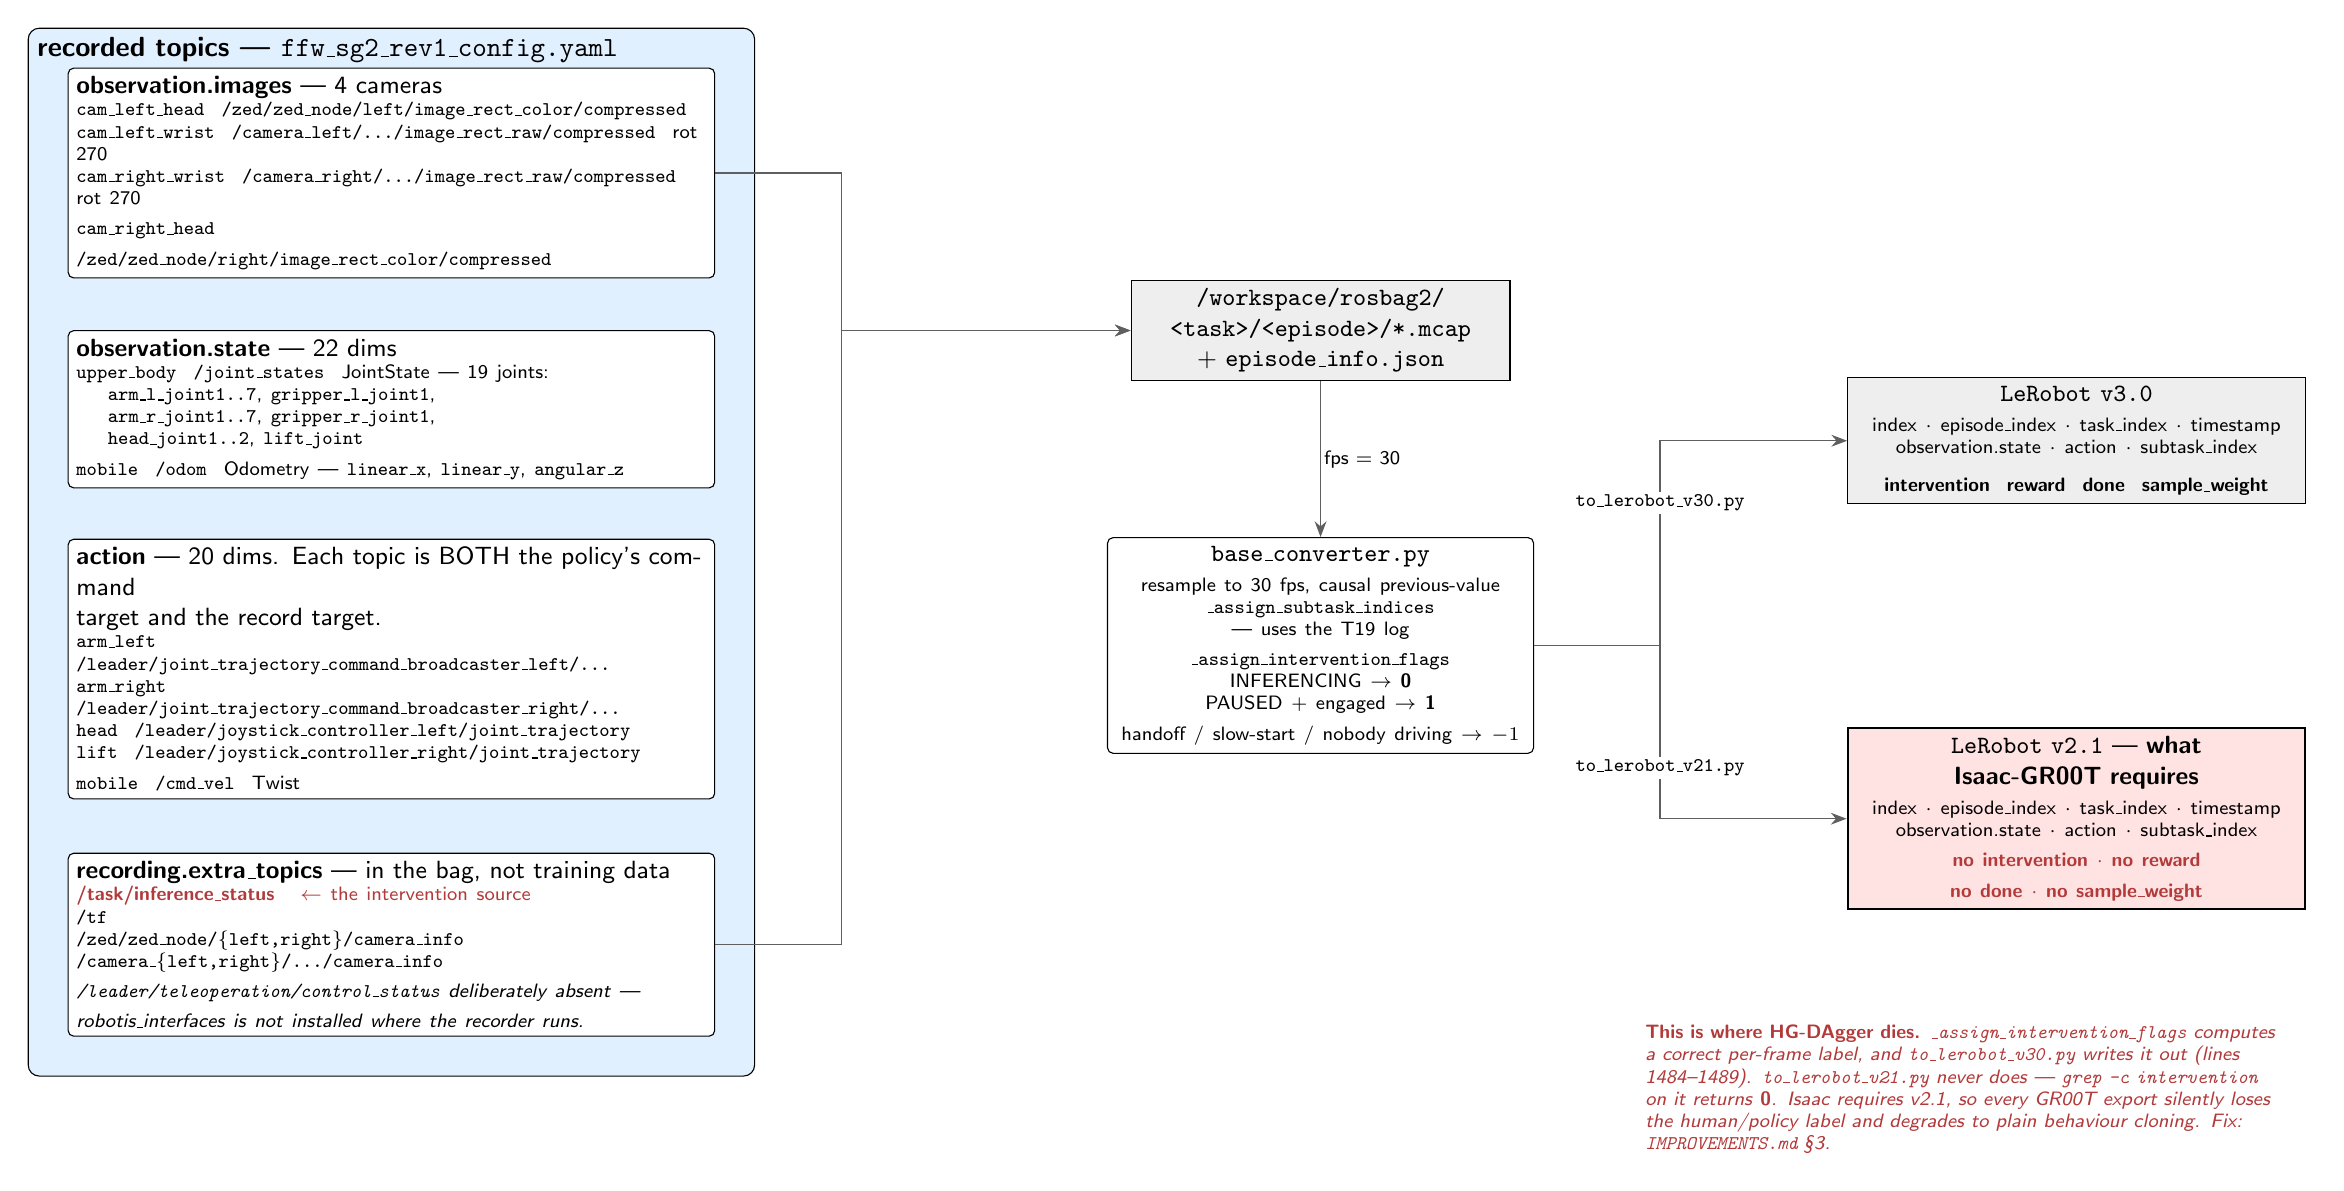
\begin{tikzpicture}[x=1cm,y=1cm]

\node[proc,text width=80mm,align=left] (obs) at (4.6,12.6)
 {\textbf{observation.images} --- 4 cameras\\
  \scriptsize\texttt{cam\_left\_head} \ \texttt{/zed/zed\_node/left/image\_rect\_color/compressed}\\
  \scriptsize\texttt{cam\_left\_wrist} \ \texttt{/camera\_left/.../image\_rect\_raw/compressed} \ rot 270\\
  \scriptsize\texttt{cam\_right\_wrist} \ \texttt{/camera\_right/.../image\_rect\_raw/compressed} \ rot 270\\
  \scriptsize\texttt{cam\_right\_head} \ \texttt{/zed/zed\_node/right/image\_rect\_color/compressed}};

\node[proc,text width=80mm,align=left] (st) at (4.6,9.6)
 {\textbf{observation.state} --- 22 dims\\
  \scriptsize\texttt{upper\_body} \ \texttt{/joint\_states} \ JointState --- 19 joints:\\
  \scriptsize\hspace{4mm}\texttt{arm\_l\_joint1..7}, \texttt{gripper\_l\_joint1},\\
  \scriptsize\hspace{4mm}\texttt{arm\_r\_joint1..7}, \texttt{gripper\_r\_joint1},\\
  \scriptsize\hspace{4mm}\texttt{head\_joint1..2}, \texttt{lift\_joint}\\
  \scriptsize\texttt{mobile} \ \texttt{/odom} \ Odometry --- \texttt{linear\_x}, \texttt{linear\_y}, \texttt{angular\_z}};

\node[proc,text width=80mm,align=left] (ac) at (4.6,6.3)
 {\textbf{action} --- 20 dims. Each topic is BOTH the policy's command\\target and the record target.\\
  \scriptsize\texttt{arm\_left} \ \texttt{/leader/joint\_trajectory\_command\_broadcaster\_left/...}\\
  \scriptsize\texttt{arm\_right} \ \texttt{/leader/joint\_trajectory\_command\_broadcaster\_right/...}\\
  \scriptsize\texttt{head} \ \texttt{/leader/joystick\_controller\_left/joint\_trajectory}\\
  \scriptsize\texttt{lift} \ \texttt{/leader/joystick\_controller\_right/joint\_trajectory}\\
  \scriptsize\texttt{mobile} \ \texttt{/cmd\_vel} \ Twist};

\node[proc,text width=80mm,align=left] (ex) at (4.6,2.8)
 {\textbf{recording.extra\_topics} --- in the bag, not training data\\
  \scriptsize\textcolor{eHuman}{\textbf{/task/inference\_status}} \ \ \textcolor{eHuman}{$\leftarrow$ the intervention source}\\
  \scriptsize\texttt{/tf}\\
  \scriptsize\texttt{/zed/zed\_node/\{left,right\}/camera\_info}\\
  \scriptsize\texttt{/camera\_\{left,right\}/.../camera\_info}\\[1mm]
  \scriptsize\itshape \texttt{/leader/teleoperation/control\_status} deliberately absent ---\\
  \scriptsize\itshape robotis\_interfaces is not installed where the recorder runs.};

\begin{scope}[on background layer]
\node[container,fill=cAiWorker,fit=(obs)(st)(ac)(ex),
      label={[font=\bfseries,anchor=north west]north west:recorded topics --- \texttt{ffw\_sg2\_rev1\_config.yaml}}] {};
\end{scope}

\node[disk,text width=46mm] (mcap) at (16.4,10.6)
 {\texttt{/workspace/rosbag2/}\\\texttt{<task>/<episode>/*.mcap}\\+ \texttt{episode\_info.json}};

\node[proc,text width=52mm] (conv) at (16.4,6.6)
 {\texttt{base\_converter.py}\\[1mm]
  \scriptsize resample to 30 fps, causal previous-value\\
  \scriptsize \texttt{\_assign\_subtask\_indices} --- uses the T19 log\\[1mm]
  \scriptsize\textbf{\texttt{\_assign\_intervention\_flags}}\\
  \scriptsize INFERENCING $\to$ \textbf{0} \ \ PAUSED + engaged $\to$ \textbf{1}\\
  \scriptsize handoff / slow-start / nobody driving $\to$ \textbf{$-1$}};

\draw[ed] (obs.east) -- ++(1.6,0) |- (mcap.west);
\draw[ed] (ex.east)  -- ++(1.6,0) |- (mcap.west);
\draw[ed] (mcap) -- node[lbl,right]{fps $=$ 30} (conv);

\node[disk,text width=56mm] (v30) at (26.0,9.2)
 {\texttt{LeRobot v3.0}\\[1mm]
  \scriptsize index $\cdot$ episode\_index $\cdot$ task\_index $\cdot$ timestamp\\
  \scriptsize observation.state $\cdot$ action $\cdot$ subtask\_index\\[1mm]
  \scriptsize\textbf{intervention} \ \textbf{reward} \ \textbf{done} \ \textbf{sample\_weight}};

\node[bad,text width=56mm] (v21) at (26.0,4.4)
 {\texttt{LeRobot v2.1} --- \textbf{what Isaac-GR00T requires}\\[1mm]
  \scriptsize index $\cdot$ episode\_index $\cdot$ task\_index $\cdot$ timestamp\\
  \scriptsize observation.state $\cdot$ action $\cdot$ subtask\_index\\[1mm]
  \scriptsize\textcolor{eHuman}{\textbf{no intervention $\cdot$ no reward}}\\
  \scriptsize\textcolor{eHuman}{\textbf{no done $\cdot$ no sample\_weight}}};

\draw[ed] (conv.east) -- ++(1.6,0) |- node[lbl,pos=0.32,above]{\texttt{to\_lerobot\_v30.py}} (v30.west);
\draw[ed] (conv.east) -- ++(1.6,0) |- node[lbl,pos=0.32,below]{\texttt{to\_lerobot\_v21.py}} (v21.west);

\node[note,text width=84mm,anchor=north west,text=eHuman] at (20.4,1.9)
 {\textbf{This is where HG-DAgger dies.} \texttt{\_assign\_intervention\_flags}
  computes a correct per-frame label, and \texttt{to\_lerobot\_v30.py} writes it out
  (lines 1484--1489). \texttt{to\_lerobot\_v21.py} never does --- \texttt{grep -c
  intervention} on it returns \textbf{0}. Isaac requires v2.1, so every GR00T export
  silently loses the human/policy label and degrades to plain behaviour cloning.
  Fix: \texttt{IMPROVEMENTS.md} \S3.};

\end{tikzpicture}}

\newpage

% =====================================================================
% PAGE 3+ -- LEGEND
% =====================================================================
{\LARGE\bfseries Topic / Service Legend}\\[1mm]
{\small Verified against \texttt{cyclo\_intelligence\_backup@main} and \texttt{aiw\_backup@feature-a2}, 2026-08-30.}\\[3mm]

{\renewcommand{\arraystretch}{1.35}
\begin{longtable}{p{9mm}p{24mm}p{76mm}p{50mm}p{196mm}}
\hline
\textbf{ID} & \textbf{Kind} & \textbf{Name} & \textbf{Type} & \textbf{Meaning / gotcha}\\
\hline
\endhead
T1 & \small PUB/SUB & \texttt{\small /leader/joystick\_controller/\allowbreak tact\_trigger} & \texttt{\small std\_msgs/String} & \small Tap emits "left"/"right". \textbf{Record trigger disabled} --- one press also engages that arm, which during INFERENCING would put the leader onto T6 against the policy.\\
T2 & \small PUB/SUB & \texttt{\small .../joystick\_command} & \texttt{\small robotis\_interfaces/\allowbreak TeleoperationCommand} & \small ENABLE / DISABLE / \textbf{TOGGLE}, per arm. The tact sends TOGGLE --- engage and stop are the same press.\\
T3 & \small PUB/SUB & \texttt{\small .../raw\_joint\_trajectory} & \texttt{\small trajectory\_msgs/\allowbreak JointTrajectory} & \small The leader's own arm command, before mode handling.\\
T4 & \small PUB/SUB & \texttt{\small /leader/teleoperation/\allowbreak control\_status} & \texttt{\small robotis\_interfaces/\allowbreak ControlModeStatus} & \small \texttt{active\_arms} + mode. Use T5.\\
T5 & \small PUB/SUB \emph{latched} & \texttt{\small /leader/teleoperation/\allowbreak active\_arms\_str} & \texttt{\small std\_msgs/String} & \small Same information as T4 as a plain string, from \texttt{leader\_bridge.py}. The UI badge reads it; \textbf{the bag should too}.\\
T6 & \small PUB/SUB & \texttt{\small /leader/joint\_trajectory\_command\_\allowbreak broadcaster\_\{left,right\}/\allowbreak joint\_trajectory} & \texttt{\small trajectory\_msgs/\allowbreak JointTrajectory} & \small \textbf{Written by BOTH the teleop node and the policy.} That is why \texttt{action} is valid in either mode. T14 prevents contention, not separate topics.\\
T7 & \small PUB/SUB & \texttt{\small /joint\_states}, \texttt{\small /odom}, 4 camera topics & \texttt{\small JointState, Odometry,\allowbreak CompressedImage} & \small Follower feedback and vision. 4 cameras recorded, 3 declared to the policy.\\
T8 & \small PUB/SUB & \texttt{\small /<backend>/engine\_command} & \texttt{\small std\_msgs/String} & \small Orchestrator $\to$ \texttt{groot\_server}: load / unload / run.\\
T9 & \small SERVICE & \texttt{\small /task/command} & \texttt{\small SendCommand.srv} & \small Start / Pause / Resume / Clear policy; Start / Stop / Cancel recording.\\
T10 & \small PUB/SUB \emph{latched} & \texttt{\small /task/inference\_status} & \texttt{\small interfaces/\allowbreak InferenceStatus} & \small \texttt{inference\_phase}: READY 0, LOADING 1, INFERENCING 2, PAUSED 3. \textbf{Transitions only} --- the converter forward-fills. Sole source of the intervention label.\\
T11 & \small SERVICE & \texttt{\small /data/recording} & \texttt{\small RecordingCommand.srv} & \small Recording lifecycle, orchestrator $\to$ \texttt{cyclo\_data\_node}.\\
T13 & \small SERVICE & \texttt{\small /data/convert}, \texttt{\small /data/convert/status} & \texttt{\small StartConversion.srv,\allowbreak GetConversionStatus.srv} & \small LeRobot conversion. Both \texttt{convert\_v21} and \texttt{convert\_v30} false means "run both".\\
T14 & \small PUB/SUB \emph{latched} & \texttt{\small /task/policy\_active} & \texttt{\small std\_msgs/Bool} & \small Mirrors T10's INFERENCING into \texttt{ai\_worker}. Gates the leader chain off T6 so the two never publish together.\\
T15 & \small PUB/SUB & \texttt{\small .../sensorxel\_joy\_values} & \texttt{\small std\_msgs/\allowbreak Float64MultiArray} & \small Raw joystick axes. The gesture detector watches these.\\
T16 & \small PUB/SUB & \texttt{\small /leader/teleoperation/\allowbreak toggle\_pause\_request} & \texttt{\small std\_msgs/Empty} & \small Fires once on a $\geq$1\,s drag-hold. \textbf{One topic, two meanings}: pause if INFERENCING, resume if PAUSED. Lets the operator work without the browser.\\
T17 & \small PUB/SUB & \texttt{\small .../control\_command} & \texttt{\small robotis\_interfaces/\allowbreak ControlModeCommand} & \small Mode 1 absolute MoveJ, mode 2 relative delta. \textbf{SG2 default is mode 2.}\\
T18 & \small PUB/SUB \emph{latched} & \texttt{\small /task/home\_in\_progress} & \texttt{\small std\_msgs/Bool} & \small One-shot Home trajectory, published \textbf{straight from the browser} --- the only UI action that skips the orchestrator.\\
T19 & \small SERVICE & \texttt{\small /task/command}\ (UPDATE\_INSTRUCTION) & \texttt{\small SendCommand.srv} & \small Appends to \texttt{instruction\_change\_log}, which splits the episode into correctly-timed sub-segments. Without it a continuous take gets one segment and every frame carries the last instruction set.\\
\hline
\end{longtable}}

\vspace{2mm}
{\large\bfseries Derived dataset columns}\\[2mm]
\begin{itemize}[leftmargin=6mm,itemsep=1.2mm]
\item \textbf{\texttt{observation.state}} (22) and \textbf{\texttt{action}} (20) --- they differ: state carries \texttt{head\_joint1/2}, action does not. Slice order follows YAML insertion order. The policy declares only the first 16 (both arms); the remainder are recorded but not trained on.
\item \textbf{\texttt{task\_index} / \texttt{subtask\_index}} --- per frame, from \texttt{episode\_info.json}'s \texttt{segments}, split by \texttt{instruction\_change\_log} (T19). The episode's top-level \texttt{task\_instruction} is a separate stable field; it is \emph{not} the live per-phase instruction, which is overwritten on every T19 click.
\item \textbf{\texttt{intervention}} --- \textbf{1 = human drove, 0 = policy drove, $-1$ = excluded} (handoff, nobody driving, phase never observed --- note the handoff rule assumes a mode-1 sweep, see \texttt{IMPROVEMENTS.md} Defect 2). This is the \emph{inverse} of \texttt{task\_is\_policy}, the name some downstream tooling expects; getting the polarity wrong raises nothing and trains on exactly the wrong frames. \textbf{v3.0 only.}
\item \textbf{\texttt{reward}, \texttt{done}, \texttt{sample\_weight}} --- emitted alongside \texttt{intervention}. \textbf{v3.0 only}, so HIL-SERL-style training is also impossible from a v2.1 export.
\end{itemize}

\end{document}
